\documentclass[tikz]{standalone}%

\usetikzlibrary{calc}
\usepackage{pgfplots}
\pgfplotsset{compat = newest}
\usepgfplotslibrary{colormaps}
\usepackage{amsmath}

\begin{document}

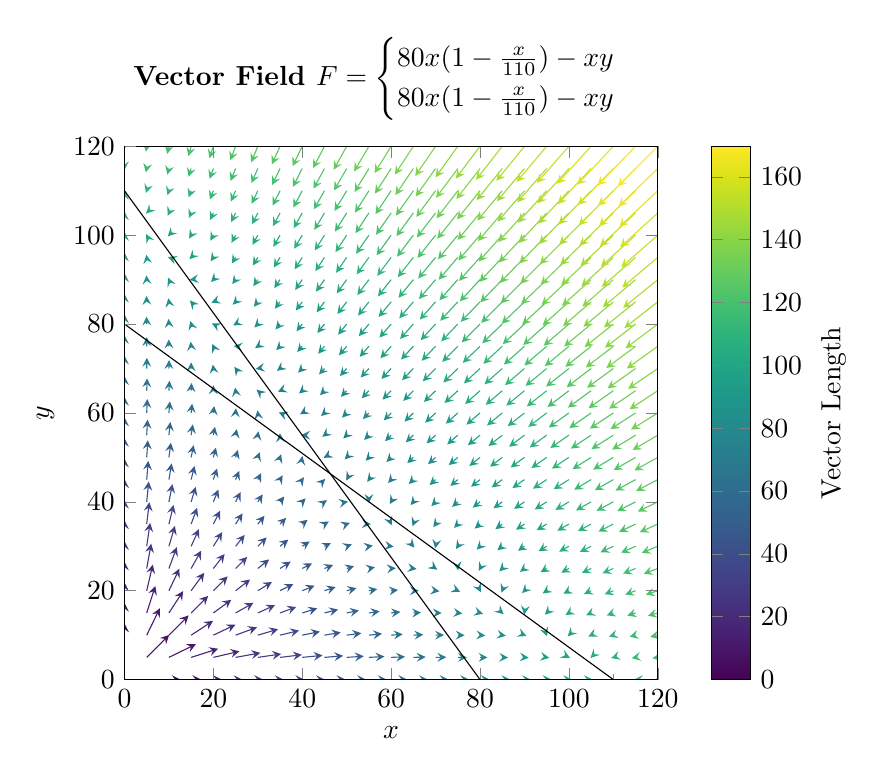
\begin{tikzpicture}
    \begin{axis}[
        xmin = 0, xmax = 120,
        ymin = 0, ymax = 120,
        zmin = 0, zmax = 1,
        axis equal image,
        xtick distance = 20,
        ytick distance = 20,
        view = {0}{90},
        scale = 1.25,
        title = {\bf Vector Field $F = 
        \begin{cases}
            80x(1 - \frac{x}{110}) -xy \\
            80x(1 - \frac{x}{110}) -xy
        \end{cases}
        $},
        height=7cm,
        xlabel = {$x$},
        ylabel = {$y$},
        colormap/viridis,
        colorbar,
        colorbar style = {
            ylabel = {Vector Length}
        }
    ]
     
    \addplot3[
        point meta = {sqrt(x^2+y^2)},
        quiver = {
            u = { ( 80 * x * (1 - x / 110) - 1 * x * y ) /sqrt(x^2+y^2)},
            v = { ( 80 * y * (1 - y / 110) - 1 * x * y ) /sqrt(x^2+y^2)},
            scale arrows = 0.10,
        },
        quiver/colored = {mapped color},
        -stealth,
        domain = 0:120,
        domain y = 0:120,
    ] {0};
     
    \draw (0,80) -- (110,0) ;
    \draw (0,110) -- (80,0) ;

    \end{axis}


\end{tikzpicture}% Further ’tikzpicture’ environments are possible which will create further pages.

\end{document}